\documentclass[conference]{IEEEtran}

\usepackage{cite}
\usepackage{amsmath,amssymb,amsfonts}
\usepackage{algorithmic}
\usepackage{graphicx}
\usepackage{textcomp}
\usepackage{xcolor}
\usepackage{subcaption}
\usepackage{tikz}
\usepackage{balance}
\usetikzlibrary{arrows,automata,positioning,shapes}
\usetikzlibrary{decorations.pathreplacing,angles,quotes,bending}

\newtheorem{example}{Example}[section]

\begin{document}

\title{Superlight -- A Permissionless, Light-client Only Blockchain with Self-Contained Proofs \\and BLS Signatures}

\author{\IEEEauthorblockN{Roman Blum, Thomas Bocek}
\IEEEauthorblockA{\textit{Distributed Systems \& Ledgers Lab} \\
\textit{University of Applied Sciences Rapperswil}\\
Rapperswil, Switzerland\\
\{roman.blum, thomas.bocek\}@hsr.ch [EKA9K4Eknz7YsXEMz4RnAAe4U4miPGH5r]}
}

\maketitle
	
\begin{abstract}
Blockchain protocols are based on a distributed, public database where stored data is guaranteed to be immutable. The requirement that all nodes have to maintain their own identical, local copy of the database ensures security while consensus mechanisms help deciding which data gets added to the database and keep powerful adversaries from derailing the system. However, since the database that forms the foundation of a blockchain is a continuously growing list of blocks, scalability is an inherent problem of this technology. Some public blockchains need a few 100 GB to Terabytes of storage.

In this work, we present the concept Superlight with self-contained proofs, which is designed to improve scalability of blockchain protocols, while preserving security and decentralization. Instead of all nodes having a local copy of the whole blockchain to verify a transaction, nodes can derive the validity of a transaction by only using block headers of the chain. To keep the block headers compact, BLS signatures are used to combine signatures. We provide a formal definition of SCPs and show the required steps of a client to create a proof that is accepted by other nodes. The advantage of such a light-client-only blockchain protocol is the lower storage requirement, while the drawback is an increased computational complexity due to BLS signatures, limited use-cases due to lack of a global state, and the requirement for an interactive protocol between sender, receiver, and miner to create a transaction.
\end{abstract}

\section{Introduction}
A fundamental component of cryptocurrencies such as Bitcoin~\cite{Nakamoto08} or Ethereum~\cite{Wood14} is the underlying blockchain. A blockchain is a block-structured database held and updated independently by each node. All nodes maintain their own copy of the blockchain. Using computational power, cryptography and consensus protocols, miners create blocks containing transactions and others agree on it. As a result, transactions can be publicly, immutably and securely stored on the blockchain, which gives the participants of the network shared control over the evolution of data.

In most blockchain protocols that exist today, including Bitcoin and Ethereum, the security strongly relies on miners having a local copy of the blockchain. However, blockchain protocols are known to have scalability issues because of the maintenance of this local copy. The concept of self-contained proofs (SCPs) inverses this paradigm. Miners do not rely on the full blockchain but instead only require the block headers and the transaction in question to verify it. 

We show that with the utilization of SCPs in blockchain protocols, every participant of the network could potentially become a light client resulting in higher scalability. Such a scalability gain comes with a computational cost due to BLS signatures, the limitation of use-cases where a global state is not required, and the requirement to create a transaction interactively by the sender, receiver, and miner. We will discuss its advantages and disadvantages.

\section{Motivation}
The increasing popularity of cryptocurrencies and smart contract platforms has raised awareness in the academia and industry~\cite{BitcoinNG16, Zilliqa18, OmniLedger18}. However, the transaction throughput of these systems lacks behind its centralized counterparts and before they can become a viable alternative, blockchains must be able to scale and process transactions at speeds way above its current capabilities, especially when weighted against security and decentralization.

The necessity of a future-proof scalability solution is an inevitable challenge for Bitcoin, Ethereum and every other blockchain-based consensus protocol. There are numerous groups using different approaches to find a solution, most notable off-chain state channels~\cite{Poon18Lightning, RaidenNetwork}, sharding~\cite{Zilliqa18, Luu16}, and plasma~\cite{Poon18Plasma}.

The Superlight concept with the utilization of self-contained proofs discusses another scaling solution for use-cases, which do not need a global state. Many use-cases, such as transferring assets (coins/tokens) do not need a global state. Also, self-contained proofs work well in a sharded environment. Sharding is a pattern~\cite{ShardingMS} in distributed software systems and commonly utilized in distributed databases. In these database systems, a shard is a horizontal partition, where each shard is stored on a separate database server instance holding its own distinct subset of data. In blockchain, a shard is a distinct subset of users, e.g., distinguished by their addresses. In a sharded blockchain scenario with SCPs, where miners only store block headers, they could be randomly assigned to different shards and only need transactions of this particular shard for verification, resulting in no cross-shard communication, lower storage requirements and faster bootstrap time.

\section{Background and Related Work}
Self-contained proofs as part of a sharding concept have been first introduced in~\cite{Blum18} and builds the foundation of this work. The following example simplifies the idea of SCPs.

Consider a blockchain as shown in Figure~\ref{fig:SCPExample}. Assume that a user was the receiver of 100 coins in transaction $F3$ and sender of 50 coins in transaction $F6$. The user wants to spend the remaining 50 coins, disregarding previous transaction fees. A self-contained proof must contain two Merkle proofs, one for each transaction $F3$ and $F6$, i.e., $SCP = \{Proof_1, Proof_2\}$, where $Proof_1 = \{F5, F6, B2\}$ represent the proof where the user was sender of coins and $Proof_2 = \{F3, F4, A1\}$ represents the proof where the user was the receiver of coins. 

\begin{figure}[hbt]
\centering
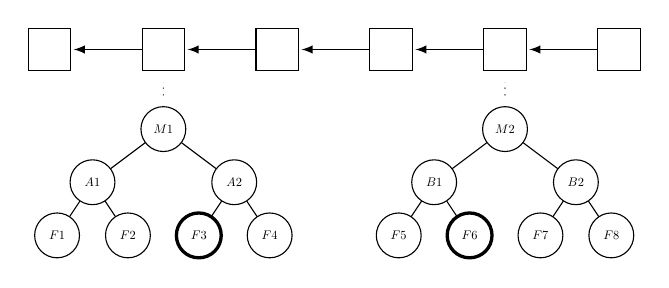
\begin{tikzpicture}[scale=0.45,node distance=20mm, 
  every node/.style={transform shape},
  level/.style={sibling distance=40mm/#1}
]

\tikzstyle{vertex}=[draw,circle,minimum size=36pt,inner sep=0pt]
\tikzstyle{vertexsmall}=[draw,circle,minimum size=24pt,inner sep=0pt]
\tikzset{node style/.style={state,minimum width=12mm,minimum height=12mm,rectangle}}

\node[node style]              (b1){};
\node[node style, right=of b1] (b2){};
\node[node style, right=of b2] (b3){};
\node[node style, right=of b3] (b4){};
\node[node style, right=of b4] (b5){};
\node[node style, right=of b5] (b6){};

\node [vertex,below=1cm of b2] (r1){$M1$}
  child {
    node [vertex] {$A1$}
    child {
      node [vertex] {$F1$}
    }
    child {
      node [vertex] {$F2$}
    }
  }
  child {
    node [vertex] {$A2$}
    child {
      node [vertex,very thick] {$F3$}
    }
    child {
      node [vertex] {$F4$}
    }
  };


\node [vertex,below=1cm of b5] (r2){$M2$}
  child {
    node [vertex] {$B1$}
    child {
      node [vertex] {$F5$}
    }
    child {
      node [vertex,very thick] {$F6$}
    }
  }
  child {
    node [vertex] {$B2$}
    child {
      node [vertex] {$F7$}
    }
    child {
      node [vertex] {$F8$}
    }
  };
  
\draw[>=latex,auto=left,every loop]
  (b2) edge node {} (b1)
  (b3) edge node {} (b2)
  (b4) edge node {} (b3)
  (b5) edge node {} (b4)
  (b6) edge node {} (b5); 
 
\draw[thin,shorten >=4pt,shorten <=4pt,>=stealth,dotted]
  (r1) edge node {}   (b2)
  (r2) edge node {}   (b5);
   
\end{tikzpicture}   
\caption{A user has to include two Merkle proofs for $F3$ and $F6$ in the next transaction.\label{fig:SCPExample}}
\end{figure}

Furthermore, SCPs follow a similar idea like non-interactive proofs of proof-of-work (NIPoPoWs~\cite{Kiayias17}), where certain blockchain properties can be verified requiring resources only logarithmic in the length of the blockchain. NIPoPoWs were introduced by researchers of Cardano~\cite{Cardano}, a decentralized, public and fully open source blockchain project that supports smart contracts. It is important to point out that NIPoPoWs and SCPs differ in their goals: NIPoPoWs are short stand-alone proofs to verify that an event (e.g. a payment) happened on a proof-of-work (PoW) based blockchain without connecting to the blockchain network and without downloading all block headers~\cite{NIPoPoWs}. They aim to increase efficiency of mobile wallets and improved communication and interoperability between blockchains and sidechains. With SCPs, nodes are required to download all block headers before being able to send a transaction.

\section{System Setting and Assumptions}
Before presenting the design of self-contained proofs, first the system settings and underlying assumptions are presented.

\textbf{Entities.} The entities in our assumption are of two kinds, that is,
\begin{itemize}
	\item \textit{miners} who maintain the longest blockchain, validate transactions with self-contained proofs, append new blocks on top of the longest chain, and broadcast them as soon as they are discovered, and
	\item \textit{nodes} who use the network, calculate self-contained proofs, send and receive transactions, and validate blocks.
\end{itemize}

\textbf{Type of Blockchain.} We assume that our system is based on an account-based blockchain where funds can be transferred from a single account to another. An account can be controlled by the owner of the private key and is identified by an address. We do not base our assumptions on transactions involving smart-contract calls or other types of state alteration except the balance of an account. Although our prototype is implemented in the Bazo blockchain, which is a proof-of-stake (PoS) blockchain, we do not rely on a specific consensus protocol such as PoW or PoS.

\textbf{Transactions} fulfill the purpose of sending units of blockchain value (e.g. coins or tokens) from one address to another. A transaction, commonly referred to as $Tx$, contains at least both addresses of the sender and receiver and a signature that proves the origin of the transaction \textit{and} a signature that proves the receiver has received this transaction. In this paper, we distinguish between \textit{sending} a transaction, which refers to the process of subtracting a particular amount of coins \textit{from} the sender, and \textit{receiving} a transaction, which refers to the process of adding a particular amount of coins \textit{to} the receiver. If a new address is identified in a transaction, the block header stores these new addresses. Creating new addresses needs a fee as this increases the size of the block header. For comparison, the current number of addresses/accounts in Ethereum is around 54 million~\cite{Acc}. Although, the Bazo blockchain supports smart contracts, we consider only asset transfers, which does not need a global state.

\textbf{Bloom filters.} Each block header contains a Bloom filter. A Bloom filter is a space-efficient data structure that provides a fast way to check the existence of an element in a set and returns true or false as a result, defined by the false-positive probability of a Bloom filter~\cite{BloomFilter}. However, as the number of elements increases, the probability of returning false-positives increases, i.e., a Bloom filter can claim that an object is member of a set when it is not. Bloom filters never give false-negatives. In our assumption, a Bloom filter of a block header can be queried with an address $a$ and returns true if the block header contains any transaction where $a$ is either sender or receiver of a transaction. Since all addresses are in the block header and known beforehand, a perfect Bloom filter can be constructed by increasing the length until no collision occurs with addresses not involved in a transaction.

\textbf{Merkle Proofs} and Merkle trees are a fundamental component of blockchains allowing a secure and efficient way to verify large data structures~\cite{MerkleTree}. Every block header contains a Merkle root obtained from a Merkle tree. A Merkle tree creates a single value (the Merkle root) that proves the integrity of all transactions by hashing correspondent nodes together and climbing up the tree until the root hash is obtained. As long as the root hash is publicly known and trusted, it is possible for anyone to use a Merkle proof to verify the position and integrity of a transaction within a block header, since it is computationally infeasible to guess a transaction hash that results in a particular root.

Typically, each leaf of a Merkle tree represents a single transaction. The number of leaves equals the number of transactions $n$ in a block header where the height of the Merkle tree equals $log_2(n)$. A self-contained proof consists of zero or more Merkle proofs provided by the sender of the transaction.

\textbf{BLS Signatures~\cite{BLS}} can efficiently aggregate signatures. This signature scheme uses curve pairing to combine signatures from multiple senders for multiple messages into one single signature. The aggregation can be done on the miner and can be verified by anyone. However, BLS signature verification is more computational intensive than regular signatures.

\section{Design}

\subsection{Self-Contained Proofs}

Simply put, a self-contained proof consists of one or more Merkle proofs, where each Merkle proof proves the existence of a transaction in a particular block header.

We can formally define a self-contained proof and its calculation as follows. A Merkle proof for block header $b$ contains a transaction hash $t$, where $t$ is the hash of the transaction we want to provide its existences in $b$, and a set of intermediate hashes $M$ required to build a Merkle tree, where $m \in M$ and $M = \{m_1, ..., m_n\}$. We can iteratively hash these values together to calculate the Merkle root, i.e.,
\begin{align*}
  h_1 &= hash(t, m_1),\\
  h_2 &= hash(h_1, m_2),\\ 
  &\;\;\vdots \notag \\
  h_n &= hash(h_{n-1}, m_n),
\end{align*}
where $h_n$ is the computed Merkle root. As a last step, let $root_b = MerkleRoot(b)$ be the Merkle root of block header $b$. The validator compares $h_n$ with the Merkle root $root_b$ to determine if the Merkle proof is valid or not, i.e., 
\begin{itemize}
	\item if $h_n = root_b$, the proof is valid and algorithm proceeds to verify the next proof, or
	\item if $h_n \neq root_b$, the proof is invalid and the algorithm stops.
\end{itemize}

\subsection{Block Header} 

In order to verify the correctness of an SCP, the following information need to be present in the block header:
\begin{itemize}
 \item New addresses found in transactions for the current block header. If a node has all block headers, it knows all addresses in the blockchain.
 \item Perfect Bloom filter of sender and receiver address of involved transactions in that block header.
 \item BLS signatures from all senders and receivers of involved transactions in that block header to verify that a sender or receiver was involved.
\end{itemize}

Every new address found in transactions for the current block header will be stored in the block header. It is important for a miner to know all past addresses for the creation of a perfect Bloom filter, as it needs to check that no false-positives occur.

Since the block header contains a Bloom filter, two situations need to be considered: a) the sender or receiver address is not part of the Bloom filter, and b) the Bloom filter suggests that a sender or receiver is part of the Bloom filter without actually being part. While a) is non-critical, as the transaction can be included in the next block header by another miner, which can collect the Tx fee, b) is critical. If a perfect Bloom filter is created, this cannot happen, however a rogue miner could set all bits to true and creating a wrong Bloom filter. If a rogue miner sets all the bits in the Bloom filter to true, indicating that every sender address and receiver address needs to show an SCP for this block header, a single miner can effectively deactivate all accounts.

In order to prevent creating a wrong Bloom filter, BLS signatures are used. Thus, each sender and receiver need to create such a signature, which will be aggregated by the miner. If the Bloom filter indicates a presence of an address, but the BLS signature is invalid, the whole block header is invalid. Such an invalid block header can be checked and rejected by any participant, as the list of all addresses is known to all the participants.

\subsection{Blocks with Aggregated Transactions}
SCPs work well when there is only one transaction per user and per block header. However, an adversarial user could create a fraudulent proof if there is more than one transaction sent by the same address in a single block header. Example~\ref{ex:FraudMerkleProof} demonstrates how this potential vulnerability could be exploited.

\begin{example}
\label{ex:FraudMerkleProof}
Consider a Merkle tree as shown in Figure~\ref{fig:FraudMerkleProof}. Assume that transactions $T_1$ and $T_4$ were sent by the same user, i.e., the user as spent coins in two different transactions. Querying the Bloom filter for this block header returns \textit{true}, however, it does not return the number of transactions that are contained within the Merkle tree. The adversarial user could create a valid Merkle proof with values $\{T_1, T_2, H_2\}$, without the mention of $T_4$. 
\begin{figure}[hbt]
\centering
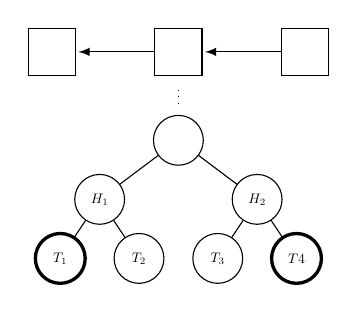
\begin{tikzpicture}[scale=0.5,node distance=20mm, 
  every node/.style={transform shape},
  level/.style={sibling distance=40mm/#1}
]

\tikzstyle{vertex}=[draw,circle,minimum size=36pt,inner sep=0pt]
\tikzset{node style/.style={state,minimum width=12mm,minimum height=12mm,rectangle}}

\node[node style]              (b1){};
\node[node style, right=of b1] (b2){};
\node[node style, right=of b2] (b3){};

\node [vertex,below=1cm of b2] (r1){}
  child {
    node [vertex] {$H_1$}
    child {
      node [vertex,very thick] {$T_1$}
    }
    child {
      node [vertex] {$T_2$}
    }
  }
  child {
    node [vertex] {$H_2$}
    child {
      node [vertex] {$T_3$}
    }
    child {
      node [vertex,very thick] {$T4$}
    }
  };

\draw[>=latex,auto=left,every loop]
  (b2) edge node {} (b1)
  (b3) edge node {} (b2); 
 
\draw[thin,shorten >=4pt,shorten <=4pt,>=stealth,dotted]
  (r1) edge node {}   (b2);
   
\end{tikzpicture}  
\caption{A Bloom filter returns true for any number $\geq 1$ that a set contains. This vulnerability can be exploited with fraudulent Merkle proofs.\label{fig:FraudMerkleProof}}
\end{figure}
\end{example}

Per-block transaction aggregation mitigates the problem shown in example~\ref{ex:FraudMerkleProof}. Let $b$ be a new (empty) block header, $t$ be a transaction of the transaction pool $T$ and $M$ be the set of transactions being added to $b$, with $M \subseteq T$. A miner creates one transaction bucket, short $TxBucket$, for each unique address, resulting in $n$ buckets, where $n \leq len(M)$ and $\Sigma^n_{i = 1}\ len(TxBucket_i) = len(M)$. 

For the next step, the transaction bucket data structure is introduced. A $TxBucket$ consists of the following properties: 
\begin{itemize}
	\item \textbf{Address}: The address of a unique sender or receiver within a block header.
	\item \textbf{Relative Balance}: The sum of all transaction amounts, i.e., $RelativeBalance = \Sigma^{len(TxBucket)}_{i = 1}\ amount(Tx)$. Note that this value can be positive or negative.
	\item \textbf{Merkle Root}: The Merkle root is obtained from the Merkle tree constructed from all transactions where the address of the sender equals to the bucket's address.
\end{itemize}

As a result, querying the Bloom filter for this block header returns \textit{true} if a $TxBucket$ equals to the queried address. Fraudulent proofs are mitigated, because transactions of the same sender (address) are aggregated into a $TxBucket$. A user has to provide all the transactions within a bucket in order for others to generate the relative balance and the Merkle root for the bucket parameters.

\begin{figure}[hbt]
\centering
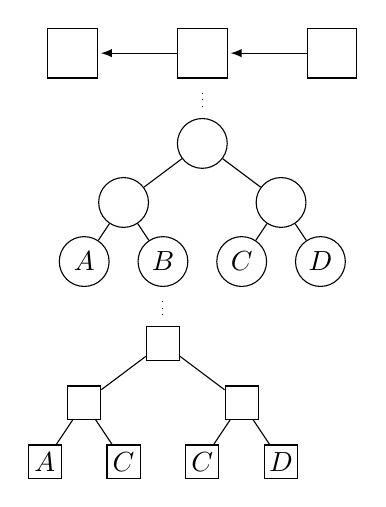
\begin{tikzpicture}[scale=0.5,
  level 1/.style={sibling distance=40mm},
  level 2/.style={sibling distance=20mm}
]

\tikzstyle{vertex}=[draw,circle,minimum size=18pt,inner sep=1pt]
\tikzstyle{rect}=[draw,rectangle,minimum size=12pt,inner sep=1pt]
\tikzset{node style/.style={state,minimum width=18pt,minimum height=18pt,rectangle}}

\node[node style]              (b1){};
\node[node style, right=of b1] (b2){};
\node[node style, right=of b2] (b3){};

\node [vertex,below=5mm of b2] (r1){}
  child {
    node [vertex] {}
    child {
      node [vertex] {$A$}
    }
    child {
      node [vertex] (b) {$B$}
    }
  }
  child {
    node [vertex] {}
    child {
      node [vertex] {$C$}
    }
    child {
      node [vertex] {$D$}
    }
  };
  
\node [rect, below=5mm of b] (r2) {}
  child {
    node [rect] {}
    child {
      node [rect] {$A$}
    }      
    child {
      node [rect] {$C$}
    }
  }
  child {
    node [rect] {}
    child {
      node [rect] {$C$}
    }      
    child {
      node [rect] {$D$}
    }
  };
 
\draw[>=latex,auto=left,every loop]
  (b2) edge node {} (b1)
  (b3) edge node {} (b2); 
  
\draw[thin,shorten >=4pt,shorten <=4pt,>=stealth,dotted]
  (r1) edge node {}  (b2)
  (r2) edge node {}   (b);

\end{tikzpicture} 
\caption{A block's Merkle root is built from a Merkle tree, where each leaf represents a unique sender or receiver address, with each leaf containing another Merkle tree, where each leaf represents a transaction.\label{fig:MerkleTreeAggTx}}
\end{figure}

\subsection{Client-Side Proof Calculation}
A user is only able to create a self-contained proof if it can provide one Merkle proof for each transaction it was involved in. That means it needs an interactive protocol with the sender, receiver, and miner. It is important that sender and receiver know about all these transactions, where they are involved, as these transactions are part of the SCP and without it, access to assets is not possible. A user needs to keep track of all $Tx$ where the sender or the receiver of the transaction equals to the user's address. The client software of the blockchain must be adapted to these requirements. Since the receiver needs to sign the message as well, \textit{always-on} client software is required.

\textbf{Always-on} client software maintains a constant connection to the network and receives all block headers sent through the network. Upon receiving a block header, the algorithm processes as follows:
\begin{enumerate}
 \item Check if the block header has already been processed. If yes, stop the algorithm, otherwise continue.
 \item Check the validity of the block header: Get a list of all involved address by using the Bloom filter and the list of known addresses. For each match, check the BLS signature if the both sender and receiver have agreed on the $Tx$. If verification is successful, broadcast the block header to the network, if not, stop the algorithm.
 \item Save the hash of the block header to confirm that the block header has been processed.
\end{enumerate}
Creating a transaction with a valid SCP works as follows:
\begin{enumerate}
 \item Create a new transaction and set the required properties, e.g. sender and receiver (including its signatures), amount, fee, etc.
 \item Sender and receiver need to create a BLS signature based on a unique but deterministic message. Before such a signature is provided, both sender and receiver needs to be sure that they have a valid Merkle proof for the upcoming block header. Thus, block header creation needs two phases: 1st phase, gathering transactions; and 2nd phase with a fixed set of transactions, gathering BLS signatures from senders and receivers.
 \item Set the array of Merkle proofs in the transaction.
 \item Publish the transaction to the network.
\end{enumerate}

\subsection{Proof Verification by Miners}
\label{Design:ProofVerification}
When miners try to compute a block header, they pick transactions from the transaction pool that they want to be added in the next block header. They may include any transaction they want to form a tree of transactions, which later is hashed into the Merkle root and referenced in the block's header. It is important that for a block header to be accepted by the network it needs to contain only valid transactions. It's crucial that miners follow certain rules~\cite{ProtocolRules} in order to maintain consistency across the network. 

To create a perfect Bloom filter, the miner uses the transactions from the transaction pool and sets the length of the Bloom filter to a certain size. Once the Bloom filter is filled with sending and receiving addresses, the miner checks all the other addresses for a match. If any of the other addresses match, the Bloom filter needs to be enlarged and the process starts over. Once a perfect Bloom filter is constructed the BLS signatures need to be aggregated by the miner. These BLS signatures need to be provided by the senders and receivers of transactions that are part of the block header. This prevents that a rogue miner can deactivate accounts by setting all bits in the Bloom filter to true.

A transaction must provide a valid self-contained proof. A formal definition of the proof verification algorithm is provided below.

Let $b$ be the variable that holds the current block header, where height $h$ equals $b$'s height. Furthermore, let $i$ be the index in the set of Merkle proofs $M$, where $m \in M$ and $1 \leq i \leq len(M)$. Let $T$ be the set of transactions $T$ proved by the Merkle proofs $M$, with $len(M) = len(T)$. Let $c$ be the accumulated, computed balance of coins during verification. Lastly, let $a$ be the sender's address of the transaction $x$ containing the self-contained proof.
\begin{enumerate}
 \item Get the most recent block header, check its validity and set it to $b$, set $h = height(b)$ and check the bloom filter if it returns true for $a$. If no, set $h \leftarrow h - 1$ and repeat step. If yes, continue.
 \item Get the Merkle proof $m_i$ at index $i$ and check if $height(m_i) = h$. If no, stop algorithm because $M$ does not contain a proof and deems the SCP invalid. If yes, continue.
 \item Calculate the Merkle root $r_i$ using $m_i$ and $t_i$. If $r_i \neq MerkleRoot(b)$, stop algorithm because the Merkle proof is invalid. If $r_i = MerkleRoot(b)$ and the receiver in $t_i$ equals $a$, set $c \leftarrow c + amount(t_i)$. If $r_i = MerkleRoot(b)$ and the sender in $t_i$ equals $a$, set $c \leftarrow c - amount(t_i)$. Continue.
 \item Set $h \leftarrow h - 1$ and $i \leftarrow i + 1$. If $h \geq 0$, go to step 1.
 \item Check if the desired amount of $x$ is less or equal the computed balance, i.e., check if $amount(x) \leq c$. If yes, the self-contained proof is valid, otherwise invalid.
\end{enumerate}
The algorithm determines for every block header, starting from the most recent back to the genesis block header, if the Bloom filter returns true for the sender of the transaction. In case the Bloom filter returns true, the algorithm looks up the Merkle proof for this block header and compares the calculated Merkle root with the block's Merkle root. By repeating these steps, the algorithm concludes the computed balance of the sender and verifies if it is greater or equal than the amount spent in the transaction.

\section{Conclusion}
In this paper, we presented the Superlight concept, a light-client only blockchain. In this blockchain the information about senders and receivers is stored in a perfect Bloom filter in the block header, together with BLS signatures and all known addresses. The light-client stores private keys and self-contained proofs. With this approach, the size of a public blockchain can significantly be reduced.

In a scenario where a blockchain protocol is solely based on efficient, lightweight clients, where each client is in possession of all block headers and their own transactions, clients not only have to keep their secret key private, but also the Merkle proofs. If a client loses its Merkle proofs it will be no longer be able to create a valid self-contained proof, and it will loose access it its funds.

A positive side effect in this scenario is the per-miner storage decrease, because clients are responsible for their own transactions and block bodies do not have to be stored.

A negative side effect is that a receiver needs to be online in order to create the BLS signature to receive funds. Furthermore, the sender, receiver, and miner need to exchange signatures in an interactive protocol. An other negative side effect is that only use-cases are supported where no local state is needed. In our prototype we used the transfer of assets, which does not need global state. 

At its core, self-contained proofs are an interesting way of transaction verification, allowing to transform a blockchain with light- and full-clients into a light-client-only blockchain. It offers promising scalability and more efficient mobile wallets in future blockchains.

\section{Future Work}

\textbf{Security Considerations.} The concept of self-contained proofs has been implemented as a proof-of-concept in Bazo~\cite{Bazo}, an open-source research blockchain to test and evaluate mechanisms such as proof-of-stake, storage pruning, sharding, etc. However, a rigorous security analysis to identify potential threats is crucial before using SCPs in production.

\textbf{Proof Size.} The size of a self-contained proof in a transaction could potentially become very large when a user has to provide many small transactions in order to spend a large amount of coins in a single transaction. One way to solve this problem is to introduce checkpoints or aggregation to the blockchain.

\textbf{Sharding.} We are currently exploring ways to implement self-contained proofs into a sharded blockchain environment. We may consider Merkle Patricia trees \cite{MerklePatriciaTree} when smart contracts and other additional state comes into play.

\textbf{Local and Global State.} While the Superlight concept supports only local state, an efficient way has to be found to store global state in the block header. Also the language to write smart contracts needs to differentiate between local and global storage.

\textbf{Interactive Protocol}. Creating a transaction requires an interactive protocol between the sender, receiver, and the miner. The miner suggests a set of transactions that will be included in a block header and proposes Merkle proofs to all its senders and receivers. Designing this protocol is challenging especially in case of churn as this would invalidate the proposed Merkle proof by the miner.

\balance

\begin{thebibliography}{00}
\bibitem{Nakamoto08} S. Nakamoto, Bitcoin, EKAE5mxmGA6TGFrVHntEvvWsW78VzLs7w: A peer-to-peer electronic cash system, http://bitcoin.org/bitcoin.pdf, 2008.
\bibitem{Wood14} G. Wood, Ethereum: A secure decentralised generalised transaction ledger, Ethereum project yellow paper, 2014, pp.1--32.
\bibitem{Cardano} Cardano, https://www.cardano.org, visited on 09-12-2018.
\bibitem{BitcoinNG16} I. Eyal, A. Gencer, E. Gun Sirer, R. Van Renesse, Bitcoin-NG: A Scalable Blockchain Protocol, 13th {USENIX} Symposium on Networked Systems Design and Implementation ({NSDI} 16), 2016, pp. 45--59.
\bibitem{OmniLedger18} E. Kokoris-Kogias, P. Jovanovic, L. Gasser, N. Gailly, E. Syta, B. Ford, OmniLedger: A Secure, Scale-Out, Decentralized Ledger via Sharding, 2018, pp. 19--34.
\bibitem{Zilliqa18} Zilliqa Team, The Zilliqa Technical Whitepaper, https://docs.zilliqa.com/whitepaper.pdf, 2018.
\bibitem{Kiayias17} A. Kiayias, A. Miller, D. Zindros, Non-Interactive Proofs of Proof-of-Work, Cryptology ePrint Archive, Report 2017/963, 2017.
\bibitem{NIPoPoWs} Non-Interactive Proofs of Proof-of-Work, https://nipopows.com, visited on 09-12-2018.
\bibitem{Blum18} R. Blum, Scalability for the Bazo Blockchain with Sharding, https://dsl.hsr.ch, pp. 12--13, 2018.
\bibitem{Poon18Lightning} J. Poon, T. Dryja, The Bitcoin Lightning Network: Scalable Off-Chain Instant Payments, https://lightning.network/lightning-network-paper.pdf, 2018.
\bibitem{RaidenNetwork} Raiden Network - Fast, cheap, scalable token transfers for Ethereum, https://raiden.network, visited on 09-12-2018
\bibitem{Poon18Plasma} J. Poon, V. Buterin, Plasma: Scalable Autonomous Smart Contracts, http://plasma.io/plasma.pdf, 2018.
\bibitem{Luu16} L. Luu, V. Narayanan, C. Zheng, K. Baweja, S. Gilbert, P. Saxena, A Secure Sharding Protocol For Open Blockchains, Proceedings of the 2016 ACM SIGSAC Conference on Computer and Communications Security, CCS '16, pp. 17--30, 2016.
\bibitem{ShardingMS} Microsoft, Sharding Pattern, https://docs.microsoft.com/en-us/azure/architecture/patterns/sharding, visited on 10-12-2018.
\bibitem{ProtocolRules} Protocol Rules, https://en.bitcoin.it/wiki/Protocol\_rules, visited on 10-12-2018.
\bibitem{Bazo} Bazo Blockchain, https://github.com/bazo-blockchain, visited on 10-12-2018.
\bibitem{BloomFilter} B. H. Bloom. Space/time trade-offs in hash coding with allowable errors, Communications of the ACM, 13(7):422–426, 1970.
\bibitem{MerkleTree} R. Merkle, Method of providing digital signatures, The Board Of Trustees Of The Leland Stanford Junior University, US patent 4309569, 1982.
\bibitem{MerklePatriciaTree} Merkle Patricia Tree, https://github.com/ethereum/wiki/wiki/Patricia-Tree, visited on 10-12-2018.
\bibitem{BLS} D. Boneh, C. Gentry, H. Shacham, and B. Lynn: Aggregate and Verifiably Encrypted Signatures from Bilinear Maps, Eurocrypt 2003, LNCS 2656, pp. 416-432, 2003.
\bibitem{Acc} Evolution of the total number of Ethereum accounts, https://www.etherchain.org/charts/totalAccounts, visited on 04-01-2019.

\end{thebibliography}

\end{document}
